% ---
% Capitulo de revisão de literatura
% ---


\chapter{Referencial Teórico}\label{referencial_teorico}
	
		\section{História do Autismo}
		Pensando nos estudos em torno da temática, organizando-os em uma linha do tempo, o termo autismo surgiu pela primeira vez em 1908, com o psiquiatra suíço Bleuler, onde ele descreveu um grupo de sintomas relacionados à esquizofrenia.
		
		Anos após as definições de Bleuler, em 1943 o psiquiatra Leo Kanner publica sua obra "Distúrbios Autísticos do contato afetivo", posteriormente os estudos passam a contemplar ou visualizar o autismo dando enfase ao isolamento extremo do indivíduo, tendo em vista a observação de traços peculiares na dificuldade de interação com outras pessoas e essa limitação perpassa também pelos elementos constituintes do ambiente, pois o autismo passa a ser contemplado nas suas dificuldades relacionadas à comunicação, resistência à mudanças, dificuldades de interação social dentre outros \cite{mcpartland2012autism}.
		
		O pesquisador e psiquiatra Hans Asperger aprofunda os estudos simultaneamente iniciado por Kanner abordando aspectos importantes para a compreensão do autismo, enfatiza que a síndrome ocorre principalmente em meninos e tem como sintomas observáveis a falta de empatia, dificuldade em relacionamentos, limitação na linguagem, dentre outros, dai percebe-se que tais questões passaram a ter uma abordagem mais ampla e ponal, pois Asperger além de reconhecer as dificuldade do autismo, faz abordagens em seus estudos sobre as capacidades apresentadas com relação a absorção de determinados conhecimentos, visto que os mesmos se estimulados nos aspectos comportamental e educacional são capazes de aprender \cite{mcpartland2012autism}.
		
		Depois desses estudos surgiram vários movimentos que complementaram e facilitaram o entendimento e o trabalho com autismo. Sabe-se que algumas doenças e sintomas são descritos nos Manuais de Diagnósticos - DSM, e em  1953, o autismo era tratado em um subgrupo da esquizofrenia, e com o passar dos anos foi considerado um conflito individual, relacionado a situações não resolvidas da vida (DSM-II). Na terceira edição do Manual de Diagnóstico (1980), o autismo entrou como uma nova classe de transtorno, os Transtornos Invasivos do Desenvolvimento, destacando algumas funções cerebrais atingidas da criança com autismo. 
		Após alguns estudos, o autismo tem suas características definidas com uma melhor precisão, e no DSM-IV, que teve seu lançamento no ano de 1994, é incluído a Síndrome de Asperger. O DSM substitui “autismo infantil” com uma definição mais ampla para “Transtorno de Autismo”, e inclui uma lista de critérios diagnósticos. Porém, em 2013, no DSM-V, os subtipos dos transtornos do espectro do autismo são eliminados. Os indivíduos são agora diagnosticados em um único espectro com diferentes níveis de gravidade e o diagnóstico para autismo passa a ser definido em duas categorias: alteração da comunicação social e pela presença de comportamentos repetitivos e estereotipados.
		
		\begin{figure}[H]
			\centering
			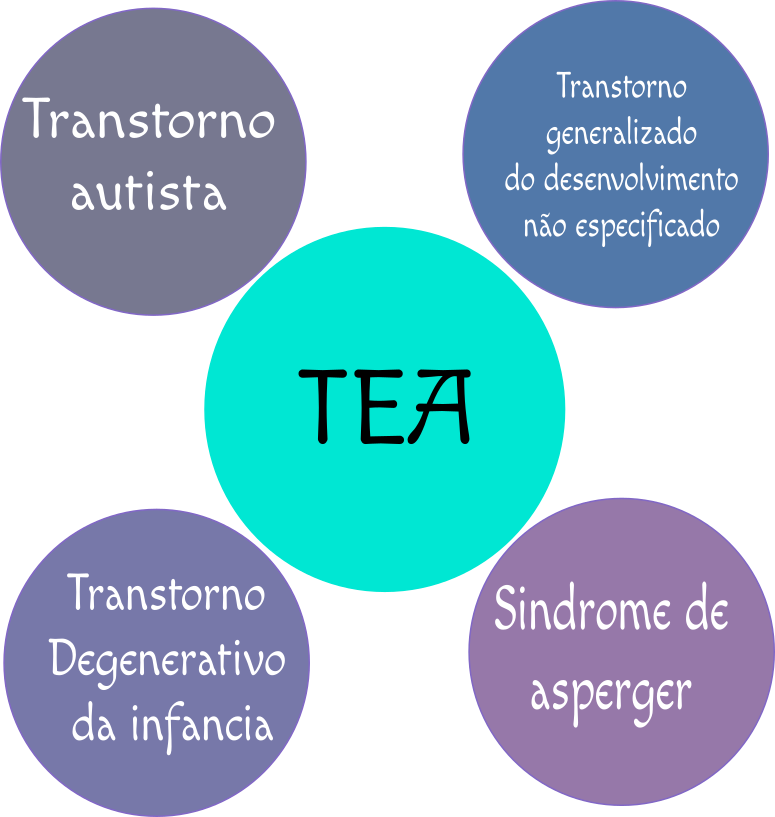
\includegraphics[scale=0.3]{img/tea-dsmv}
			\caption{Percurso do Transtorno do Espectro Autista - TEA}
			Fonte: Autor, 2018
			\label{fig:figura1}
		\end{figure}
		
		Diante da reflexão histórica abordada, verifica-se que vários estudos e pesquisas foram necessários para tornar a compreensão das características do autismo mais clara, tendo em vista as intervenções necessárias a serem adotadas. 
		%https://www.ncbi.nlm.nih.gov/pmc/articles/PMC3848246/#R93
	
		Segundo \citeonline{mello2007autismo}, o autismo é um distúrbio de desenvolvimento que se caracteriza por alterações presentes desde idades bastante precoces, normalmente se manifestam os sintomas antes dos três anos de idade, e apresentam impactos múltiplos e variados em áreas nobres do desenvolvimento humano como na comunicação, interação social, aprendizado e na capacidade de adaptação à mudanças.
		
		Em relação a descoberta da causa do transtorno, \citeonline{alcantara2013autismo}, descreve em seu estudo que houve realização de Autópsias realizadas em crianças autistas indicam que as células da região conhecida como região límbica, que é a área do cérebro que responde por emoções profundas, comportamentos sociais e por impulsos básicos, como a ira, prazer e sobrevivências, são menores e se encontram de forma mais condensada nas pessoas que apresentam o transtorno, o que indica que houve uma interrupção precoce no momento do desenvolvimento dessa parte do sistema nervoso.
		
		Porém, não há um consenso sobre o que vem a causar o autismo, muitos profissionais da saúde sugerem uma origem a partir de mutações genéticas, viroses até mesmo intoxicações por produtos químicos, dessa maneira o autismo é considerado uma síndrome, ou seja, ele é um conjunto de sintomas que podem vir a ter mais de uma única origem \cite{alcantara2013autismo}.

		Segundo \citeonline{schmidt2017transtorno}, existe a tendencia de não atribuir somente a agentes puramente ambientais ou genéticos as causas do autismo e alguns estudos apontam para fatores como: Idade avançada dos progenitores, complicações no parto e também o uso de medicamentos anti-convulsionantes e estabilizadores de humor.
		
		\citeonline{assumpccao2000autismo} cita, que o assunto de causas é adicionado pela primeira vez ao DSM em sua quarta versão, no eixo de numero 3, indica que mesmo grandes pesquisa feitas e diversos estudos sendo realizados, os dados obtidos sobre as causas não eram precisos para determinar especificamente suas causa, porém a associação com fatores biológicos era algo indiscutível.
		
		\citeonline{mesquita2013diagnostico} diz que as causa do autismo são fatores ainda desconhecido ou múltiplos fatores podem acarretar o desenvolvimento do distúrbio e os sintomas deve ser percebidos pelos responsáveis ate os três anos de idade da criança.
		
		E, diante  as incertezas ainda existentes sobre as causas, observa-se na bibliografia sobre o tema maneiras diferentes em se trabalhar com esse público.  
		\subsection{Possibilidades de intervenções} \label{tratamentos}
		%O desenvolvimento dos conceitos e formas de tratamento no decorrer da história apresentam um avanço significativo, assim a presente proposta de %estágio visa vincular as pesquisas existentes no campo da superação dos desafios enfrentados em práticas de vida diária pelos autistas às %inovações na área da tecnologia da informação, utilizando subsídios e instrumentos eficientes que auxiliam no trabalho dos profissionais que %"lidam" com crianças que tem a síndrome, bem como oportuniza o desenvolvimento gradativo da autonomia dessas crianças, no sentido de propiciar às %mesmas mais qualidade de vida, prazer e disciplina na execução de  tarefas cotidianas.     
		
		%Diante a proposta do estágio em vincular as pesquisas existentes no campo dos desafios enfrentados nas práticas de vida diária dos autistas, para %colaborar e auxiliar o desenvolvimento da autonomia das crianças com TEA, será incluído a seguir as formas de tratamento deste público, retirado %de referenciais bibliográficos. 
		
		%Nesse sentido, atualmente são utilizados elementos da gamificaçao nas terapias com autistas, no entanto, isso ocorre de forma tímida, pois as %práticas dos profissionais se restringem à bonificação simples pelos progressos nas atividades ou cumprimento das mesma.
		
		%nao cabe aqui já apresentar isso, usar la intro, fazer uma frase falandi issi, diante dessas possibilidades foi oensado nessa proposta de estágio
		 \citeonline{mello2007autismo}, expõe alguns tipos de intervenções mais usadas com as crianças TEA, como  por exemplo o TEACCH, - Tratamento e educação para crianças com autismo e distúrbio correlato da comunicação, que busca identificar os pontos fortes e dificuldades do autista, tornando possível, um programa individualizado. As intervenções aplicadas são baseadas na organização do ambiente físico, para proporcionar uma organização das tarefas da criança de modo a favorecer a independência das atividades diárias.  

		Outro mecanismo utilizado é a ABA - Análise do Comportamento Aplicado que trabalha com a criança pra que ela desenvolva habilidades por etapas, onde o mediador utiliza-se de material de apoio e à medida que nota-se avanços os recursos físicos são extintos, pois inicialmente se trabalha com estímulos para a obtenção da resposta esperada e que contribuirão com a repetição ou excursa posterior das tarefas propostas. No entanto se as respostas não forem condizentes com as premissas estabelecidas pelo profissional, ocasionando a birra ou resposta negativas por parte da criança, esta deixa de ser contemplada com o estímulo positivo. Tais resultados tem  a intenção de servir de subsídios ou análise em estudos para compreender a situação e assim evitar os comportamentos indesejados. \cite{mesquita2013diagnostico}
		
		Outra maneira de intervenção é a PECS - Sistema de comunicação através de trocas de figuras que tem a intenção de ajudar as crianças e adultos com autismo e outros distúrbios do desenvolvimento a adquirir habilidades de comunicação, com o uso de cartões que atuaram como um mediador de linguagem, deste modo, esta é estimulada a avançar se comunicando e assim através da linguagem oral a criança aprende e se torna produtiva, organizando suas falas e ações.\cite{mesquita2013diagnostico}
		
		\begin{figure}[H]
			\centering
			\includegraphics[scale=0.6]{img/materialPECS}
			\caption{Atividade no modelo PECS}
			Fonte: Mais que especial - Educação Especial Inclusiva
			\label{fig:figura4}
		\end{figure}
		
		Neste contexto percebe-se que alem do uso das estratégias acima citadas, existem outros tratamentos como o LEAP que é a Experiências de aprendizagem e programa alternativo para pré-escolares e seus pais, Denver que é o modelo inicial de denver, SCERT que significa Comunicação Social, Regulação Emocional, dentre outros. \cite{schmidt2017transtorno}.
	
	\subsection{Desenvolvimento Atípico}
	O transtorno do espectro autista pode comprometer severamente o desenvolvimento da criança que o possui, fazendo com que elas tenham algumas áreas da sua vida afetadas. \citeonline{mello2007autismo}, cita que uma área  bastante afetada, que os pais observam logo, é a comunicação, fazendo com que a criança do espectro tenha dificuldade na interação com os outros e que por esse motivo, se isole. 
	
	Segundo \citeonline{mesquita2013diagnostico}, o DSM-IV-TR aponta três principais área que pode ser observadas no momento de identificação do transtorno e que podem prejudicar na vida diária da criança autista, são elas: A área da interação social o que faz com que a pessoa não dialogue ou interaja verbalmente com outro, o total desinteresse do mesmo em convívio com pessoas da mesma idade e falta de vontade de compartilhar os prazeres ou suas realizações com outros; o uso inapropriado ou nulo da linguagem que é manifestado por meio falta da fala, dificuldade em manter discussões, ausência de imitações típicas da idade infantil e por fim os comportamentos repetitivos que é observado por rotinas imutáveis, comportamentos estereotipado e preocupação com partes de objetos.
	
	A \citeonline{de2014manual} , ainda aponta que criança com TEA apresenta falta de percepção dos acontecimentos de forma compartilhada, e prefere se concentrar em atividades isoladas. Outra característica apresentada na bibliografia disponível é a dificuldade sentimental e emocional, dificuldade em perceber e expor o que está sentindo e pensando. 
	
	Segundo \citeonline{mesquita2013diagnostico}, a maioria das crianças com autismo tem sensibilidade em um ou mais dos cinco sentidos (Audição, tato, paladar,olfato e visão), como por exemplo a hipersensibilidade auditiva, onde o portador do transtorno pode se sentir bastante incomodado com barulhos que normalmente não incomodam a outras pessoas e essas são situações que dificultam e restringem a convivência da criança.

	Para \citeonline{hobson1993autism}, as crianças com o transtorno do espectro autista tem em geral pouca ou nenhuma estratégia para compartilhar atenção com os outros. Fica claro e evidente que o processo de apropriação dessa estratégia para executar tarefas simples depende de um trabalho de mediação, onde através da utilização de novas tecnologias é possível romper as barreiras na realização dessas atividades.
	
	Dentre tais comprometimentos citados acima, o presente projeto voltará para o auxilio das intervenções diante a linguagem e as atividades de vida diária das crianças com TEA.
		
	\section{Eletronic Learning (E-Learning)}
	Segundo \citeonline{caccao2003introduccao}, o aprendizado eletrônico ou simplesmente e-learning pode ser definido como uma forma de aprendizado em que as informações e os materiais que o individuo precisa, tais como: as aulas,os documentos e a atividades de reforço, se encontra disponíveis para uso através de diversos equipamentos eletrônicos digitais, como por exemplo: os celulares, os tablets, os computadores, entre outros. 
	
	Seguindo a mesma linha de pensamento, \citeonline{clark2016learning} definem o e-learning como  conjuntos de instruções que são fornecidas por meio de um dispositivo digital, como os citados acima, os quais são destinados ao apoio à aprendizagem do individuo.
	
	Para \citeonline{gomes2005learning}, o e-learning se trata de uma extensão da sala de aula dentro de um espaço virtual na internet, isso indica que qualquer ato feito referente à atividade pedagógica em uma ambiente virtual seja definido como e-learning, desde o simples fato de disponibilizar o sumário de uma, ou aula até mesmo a realização de uma avaliação. 
	
	 \citeonline{gomes2005learning} ainda afirma que o \textit{e-learnig} pode servir como apoio ao ensino presencial, sendo que pode-se usar o \textit{e-learnig} como um complemento entre a parte presencial e à distancia, dessa forma o professor usará um ambiente virtual para: disponibilizar materiais,  auxiliar os alunos e responder dúvidas, por meio de recursos como bate-papos e fóruns.
	%https://repositorium.sdum.uminho.pt/bitstream/1822/2896/1/06MariaGomes.pdf em 02/05/18
	
	
	\citeonline{mashuda2015m} citam que embora o e-learning tenha surgido primeiramente para atender às instituições de ensino superior, ela tem crescido e se espalhado diferentes área, como por exemplo o mundo corporativo, sendo uma alternativa para treinar e especializar seus funcionários, podendo ajudar os empresários a pouparem com viagens e gastos com cursos presenciais. Tendo em vista que o e-learning está em constante crescimento, bem como a tecnologia da informação e comunicação, tende-se a surgir novas ideias, como por exemplo o conceito de m-learning, que é o uso do celular como ferramenta de aprendizado.
	%http://www.pgsskroton.com.br/seer/index.php/exatas/article/view/597/567 em 02/05/18
	
	Uma das características principais e que melhor descreve o aprendizado eletrônico, é o fato  de  que esse modelo de aprendizagem oferece uma maior facilidade e mobilidade de horários e ensino, permitindo que o tutor ou mediador esteja distante do usuário que está a usar a plataforma e-learning, permitindo então, que os alunos definam seus próprios horários para a realização das aulas. \cite{caccao2003introduccao}.
	
	Para \citeonline{caccao2003introduccao}, o \textit{e-learning } tem uma divisão básica que é baseada nos modelos pedagógicos, são eles:
	\begin{itemize}
		\item Modelo de ensino por auto-formação. É a forma de ensino-aprendizado na qual os formandos trabalham sozinhos, com uma pequena participação de seus formadores, desse modo, o próprio formando deve definir seus horários e locais de estudo e o tutor é acionado somente no momento em que o aluno tem alguma dúvida ou dificuldade com algo relativo ao material.
		
		\item Modelo de aprendizagem colaborativa. O formando é integrado em um grupo de forma virtual, onde trabalham juntos com o apoio do formador. Neste modelo são bastante utilizados as ferramentas de comunicação, como por exemplo: e-mails, fóruns e chats. Muitas vezes esta comunicação se da em tempo real.
	\end{itemize}
	
	\begin{figure}[H]
		\centering
		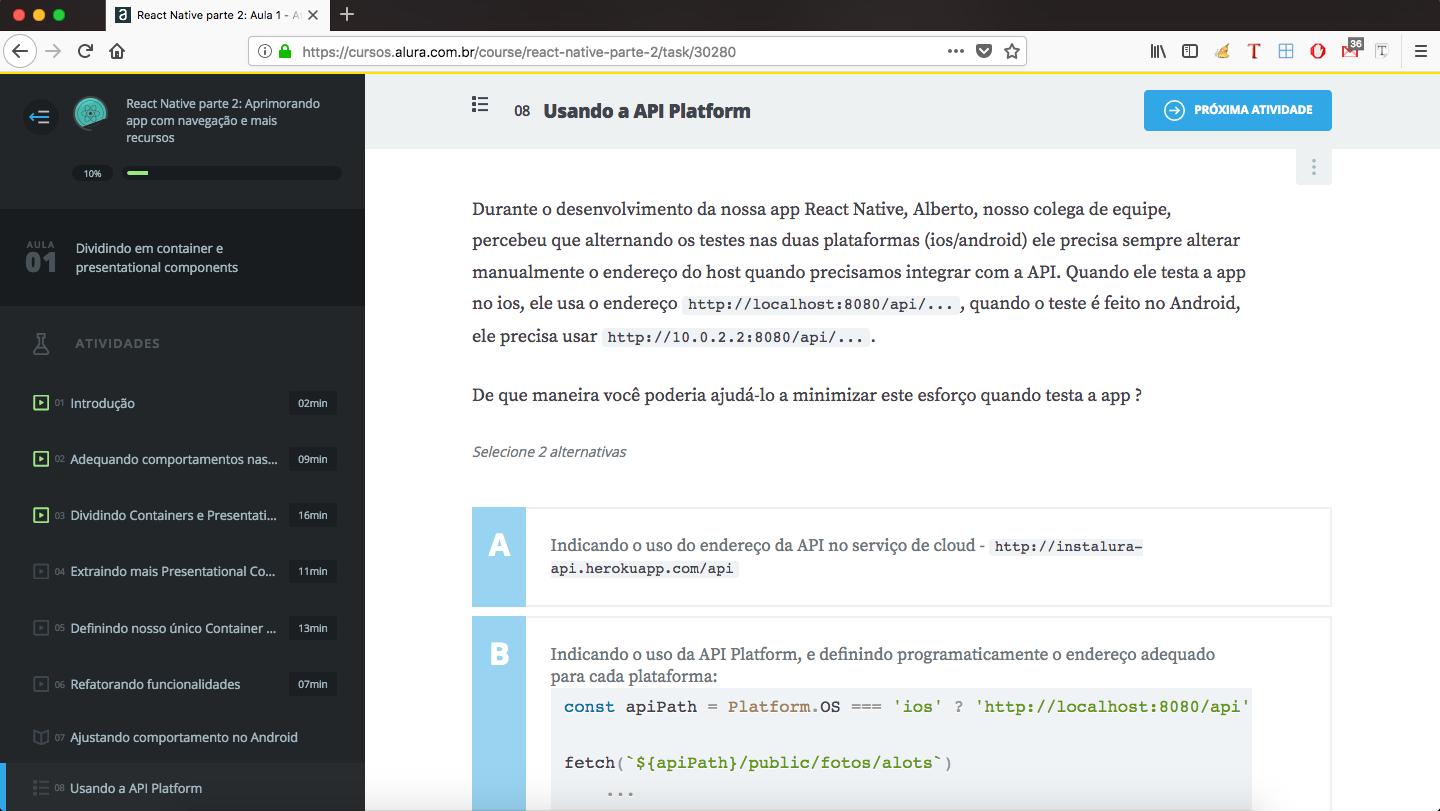
\includegraphics[width=0.6\linewidth]{img/elearningAlura}
		\caption{Plataforma de Ensino Alura}
		Fonte: Alura/Caelum
		\label{aluracaelum}
	\end{figure}

	A Figura \ref{aluracaelum} representa um exemplo de e-learning da plataforma de cursos online Alura, na qual os cursos estão divididos por aulas, e cada uma contém mídias de vídeo, textos e atividades para serem respondidas. A plataforma conta também com o um fórum que permite com que os alunos possam sanar suas dúvidas com os professores/instrutores.
	
		\subsection{Mobile Learning (M-Learning)}
 		Segundo \citeonline{pelissoli2004aprendizado}, o m-learning se trata do uso de equipamentos  celulares e tablets ligados a rede de internet, que possuam uma capacidade de manipular e visualizar mídias como fotos, voz, mensagens, e-mails e até transmissão de vídeo conferência, sendo o foco do conceito a construção de materiais atrativos e  que seja fáceis para a manipulação de quem está usando o serviço, como alunos e  treinandos.
 		%http://www.abed.org.br/congresso2004/por/htm/074-TC-C2.htm
 		
 		Para \citeonline{zanella2007m}, o m-learning basicamente se refere a aprender com mobilidade, ou seja, aprender em qualquer lugar através de um dispositivo TIMS (Tecnologia da Informação Móveis e Sem Fio), permitindo que os envolvidos no processo de aprendizagem possam estar distantes geograficamente, sem a necessidade de uma sala de aula presencial.
 		%M-LEARNING OU APRENDIZAGEM COM MOBILIDADE:	UM ESTUDO EXPLORATÓRIO SOBRE SUA UTILIZAÇÃO NO BRASIL
 		
 		\citeonline{da2013aprendizagem} cita que dentre todos os dispositivos que podem entregar ou suportar o m-learning, o mais popular e acessível é o telefone celular, o uso do mesmo para acessar aplicações m-learning se dá pela familiaridade que ele é usado, já que o mesmo se trata de uma tecnologia amigável e muito comum para o cotidiano da sociedade, o fato do mesmo ser portátil, que o permite ser levado para qualquer lugar e o fato de o mesmo poder transmitir uma ampla gama de recursos como fotos, vídeos, e-mail e outros.Os aparelhos de celular tem suas limitações, como a carga da bateria, a conexão com a internet e outros, sendo assim deve-se ter também outras formas de passar o conteúdo programado.
 		%APRENDIZAGEM, MOBILIDADE E CONVERGÊNCIA: Mobile Learning com Celulares e Smartphones
 		
 		\begin{figure}[H]
 			\centering
 			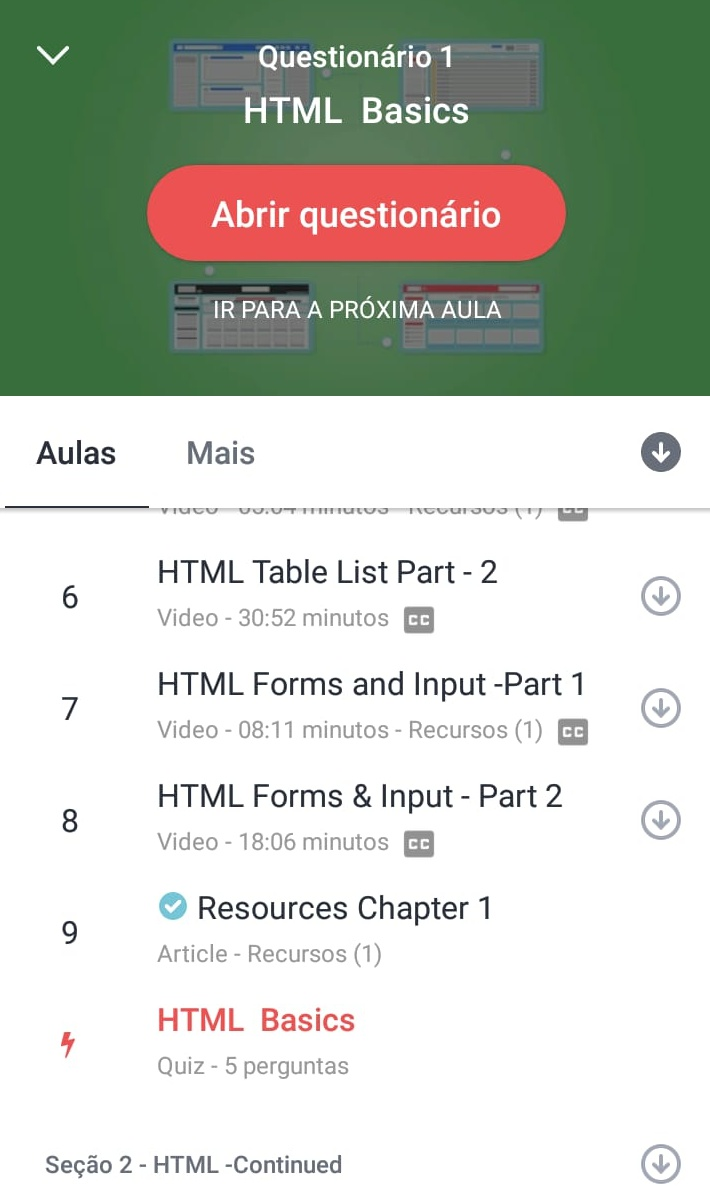
\includegraphics[width=0.4\linewidth]{img/mlearningUdemy}
 			\caption{Plataforma de Ensino Udemy}
 			Fonte: App Udemy
 			\label{udemy}
 		\end{figure}
 			A Figura \ref{udemy} mostra o aplicativo da plataforma de cursos Udemy, no qual é possível observar elementos da e-learning, como a divisão de conteúdo em aulas, e a possibilidade de acessar tanto elementos de mídia como atividades de fixação.
 		
	\section{Gamificação}
	A gamificação consiste em utilizar técnicas e mecânicas geralmente vistas em jogos para a resolução de problemas do mundo real \cite{zichermann2011gamification}. Para \cite{marczewski2013gamification}, a aplicação de elementos de jogos, em contextos fora de jogos, pode influenciar o comportamento, aumentar a motivação e melhorar o de que está participando de alguma atividade gamificada.
	
	Entender qual a motivação do jogador é o primeiro passo a tomar, ao pensar na construção de um sistema gamificado, sendo que o objeto principal em um jogo é o próprio jogador \cite{zichermann2011gamification}. Sendo assim, deve-se pensar em fatores que façam com que o usuário/jogador se sinta bem e entusiasmado ao utilizar um sistema gamificado.
	
	Para \citeonline{fardo2013gamificaccao}, a gamificação se trata de um fenômeno que ocorre por conta da alta popularização dos jogos, da capacidade que eles têm de motivar e engajar seus jogadores e a influencia global dos jogos, atingindo praticamente todas as camadas da população. 
	
			\begin{figure}[H]
				\centering
				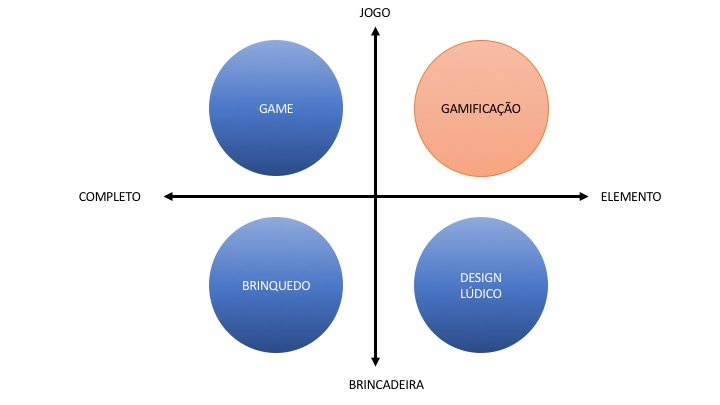
\includegraphics[width=0.7\linewidth]{img/graficoGamificacao.jpeg}
				\caption{Gráfico de Contexto da Gamificaçāo}
				Fonte: DETERDING et al.
				\label{contextoGami}
			\end{figure}
	Observando a Figura \ref{contextoGami}, que se trata de um gráfico proposto por \citeonline{deterding2011gamification}, é visto que o a gamificaçāo fica em uma área que é abrangida pelo eixo vertical que representa o jogo em si, e o eixo horizontal que representa os elementos de um jogo, onde pode-se ter o uso somente em partes.
	%http://gamification-research.org/wp-content/uploads/2011/04/02-Deterding-Khaled-Nacke-Dixon.pdf
	\subsection{Framework MDA}
	 \citeonline{zichermann2011gamification}, definem o  framework MDA(Mechanics Dynamics Aesthetics) Mecânica,Dinâmica e estética,  como uma estrutura de design de jogos bastante usada, que se baseia em três componentes, são eles: 
	 \begin{itemize}
	 	\item  A mecânica que representa os componentes funcionais do jogo, \citeonline{hunicke2004mda}, definem as mecânicas como sendo as várias ações que o jogador pode usar dentro de um jogo;
	 	
	 	\item A dinâmica, que segundo  \citeonline{zichermann2011gamification} se trata da interação do jogador  com as mecânicas do jogo, e como os jogadores estão usando as mesma, 
	 	
	 	\item A estética, que é a maneira com que o jogo faz o jogador se sentir durante sua interação com o jogo, pode-se ser visto como a criação de emoção através da integração da mecânica e dinâmica do jogo. Esses elementos podem ajudar na hora gamificar algo no mundo real.
	 \end{itemize}
	
		\begin{figure}[H]
				\centering
				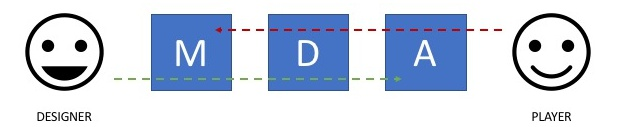
\includegraphics[width=1\linewidth]{img/pespectivasMDA}
				\caption{Diferentes Perspectivas do MDA}
				Fonte: MDA: A Formal Approach to Game Design and Game Research
				\label{visaoMDA}
		\end{figure}
	Como se pode ver na Figura \ref{visaoMDA}, o desenvolvedor do jogo, ou game design tem um determinado ponto de vista do framework MDA, pois ele ver o sistema gamificado ou mesmo jogo a partir das mecânicas, pois como o o design precisa desenvolve-las, ela se torna o ponto de partida para ele, já o jogador observa o framework a partir da estética, passando pela dinâmica e só assim depois ele observa as mecânicas do jogo.
	
	\subsection{Mecânicas de Gamificação}
	Segundo os autores  \citeonline{zichermann2011gamification}, um sistema gamificado tem sua mecânica baseada em sete elementos ou ferramentas, que ao serem utilizadas de forma correta, prometem fornecer uma resposta significativa vinda do usuário. Essas ferramentas são: pontuação, níveis, rankings, emblemas, desafios, integração e engajamento.
	
		\subsubsection{Pontos}
		A mecânica de pontos é importante para acompanhar como o jogador está se desenvolvendo dentro do jogo, por esse motivo ela é uma exigência absoluta ao se desenvolver um sistema gamificado, tanto para o jogador quanto para o desenvolvedor, sendo ela visível entre os jogadores ou somente pelo desenvolvedor, é uma importante maneira de saber como planejar e realizar os ajustes necessários,  a pontuação podem ser mostradas de forma clara, pouco visível e por fim quase invisível.\cite{zichermann2011gamification}
	   
	 \citeonline{zichermann2011gamification}, acrescentam ainda que no mundo real existem diversas formas em se utilizar a pontuação, que por serem bastante comuns, geralmente não são notadas.São citados três tipos:
	 
	 \begin{itemize}
	 	\item  A primeira é a pontuação em dinheiro, que se trata basicamente da quantidade de dinheiro que o individuo tem no banco, porém não é muito usado os números explicitamente, o que é utilizado nesse caso, são os objetos de status, que como exemplo pode-se citar as vestimentas, as viagens, os acessórios e outros.
	 	
	 	\item A segunda forma é a pontuação dos vídeo games em geral, é de fato a forma mais explícita de pontuação, a maioria dos jogos eletrônicos tem em si, sempre uma pontuação no canto da tela, indicando algo importante o quão distante ele se encontra do próximo nível, sua pontuação em relação a outros jogadores e assim por diante.
	 	
	 	\item  A terceira forma citada é a pontuação em redes sociais, que é basicamente a quantidade de amigos que a pessoa tem em uma rede social ou ainda quantos seguidores tem uma determinada página, pois quanto maior a quantidade de seguidores, maior a representatividade dentro da rede social. 
	 \end{itemize}
		
	    Na gamificaçāo pode-se utilizar cinco tipos de pontuação, sendo que nem sempre serão usados todos os tipos, são eles: pontos de experiência, pontos resgatáveis, pontos de habilidade, pontos de carma e, por fim, pontos de reputação.  \cite{zichermann2011gamification}.
	    	
		\begin{itemize}
			\item Os pontos de experiência é o tipo mais importante entre os cinco, pois identifica como o jogador está se desenvolvendo dentro do jogo, é a forma mais fácil de observar, classificar e orientar o jogador.
			
			\item Os pontos resgatáveis é basicamente a economia virtual, geralmente são relacionadas com nomes como: \textit{cash} (dinheiro), moeda, dentre outros e são utilizados  para adquirir itens dentro de um jogo.
			
			\item Os pontos de habilidade são atribuídos à realização de atividades específicas dentro do jogo, eles direcionam o jogador a realizarem algumas atividades ou sub-objetivos alternativos do jogo.
			
			\item Os pontos de Karma é o menos utilizado em sistemas gamificados, geralmente é usado para criar um caminho comportamental do jogador, servindo com que o jogadores recompensem uns aos outros como agradecimento.
			
			\item Por fim, tem-se os pontos de reputação, que é responsável por indicar  a confiança entre duas ou mais partes. Para conseguir esse tipo de pontuação, os jogadores precisam trabalhar para o bem da equipe, motivando o trabalho em equipe, bem como a cooperação entre os jogadores para atingir um objetivo em comum. Os pontos de reputação é considerado o mais complexo, pois não se pode garantir ou gerenciar a pontuação.
		\end{itemize}
		
		\begin{figure}[H]
			\centering
			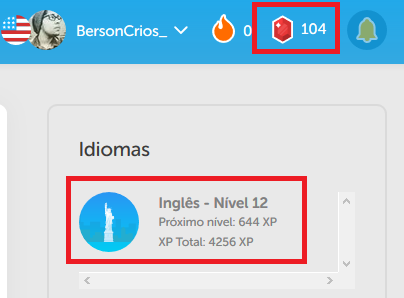
\includegraphics[width=0.5\linewidth]{img/pontosDuoLinguo}
			\caption{Ponto de Experiência e Resgatáveis no App Duolingo}
			Fonte: DuoLingo
			\label{duolingoapp}
		\end{figure}

		A Figura \ref{duolingoapp} acima representa o quadro de pontuações do aplicativo DuoLingo, pode-se notar dois tipos de pontuações que o aplicativo oferta para seus usuários conquistarem: 
		\begin{itemize}
			\item A primeira que se encontra na faixa azul, se trata dos pontos resgatáveis, são os pontos que permite com que o jogador compre itens no aplicativo.
			
			\item O segundo se trata dos pontos de experiencia, que é acumulado ao responder os desafios.
		\end{itemize}	
		
		\subsubsection{Níveis}
		Para \citeonline{zichermann2011gamification}, em um sistema gamificado, os níveis indicam progresso, porém, ao desenvolver uma experiência gamificada não se faz necessário o uso de níveis tradicionais de videogames, contudo é extremamente importante o entendimento para usá-las em sua ferramenta gamificada.
		
		Os níveis servem para auxiliar o jogador onde se encontram no jogo e não se perca ao passar algum tempo distraído com aquele jogo, essa, ao subir os níveis em um sistema gamificado, a dificuldade aumenta, porém esse aumento não é linear. \cite{zichermann2011gamification}
		
		Os arcades\footnote{Equipamento de jogos eletrônicos instalados em estabelecimento de entretenimento.} dos anos 80 tinham por interesse que os jogadores perdessem de forma mais rápida, já nos sistemas gamificados de hoje, os interesses são mais voltados a jogos mais longos e rígidos, e os níveis de dificuldade aumentam de forma gradual, do nível mais fácil ao mais difícil \cite{zichermann2011gamification}.
		
		O processo de balanceamento dos níveis é tão complexo quanto todo o processo de criação de um sistema gamificado, e é importante que sejam feitos diversos testes, mesmo com o sistema já em funcionamento. Há princípios básicos a se seguir no desenvolvimento de níveis: O primeiro principio é fazer com que o entendimento de como agir em cada nível aconteça de forma fácil para o jogador, o segundo principio é deixar com que novos níveis possam ser adicionados conforme a necessidade  de expansão apareça e, por fim, os níveis devem ser testáveis e refináveis \cite{zichermann2011gamification}.
		
		Uma representação bastante comum de visualização de progressão de níveis é através das barras de progresso, as quais permitem informar, geralmente por meio de porcentagem, o quanto o jogador já completou uma determinada etapa do que lhe foi proposto. Além de informar o quanto falta para concluir uma etapa, a barra de progresso possui a função de incentivo, ou seja, uma maneira incitar o jogador a prosseguir em sua experiência gamificada \cite{zichermann2011gamification}.
	
		\begin{figure}[H]
			\centering
			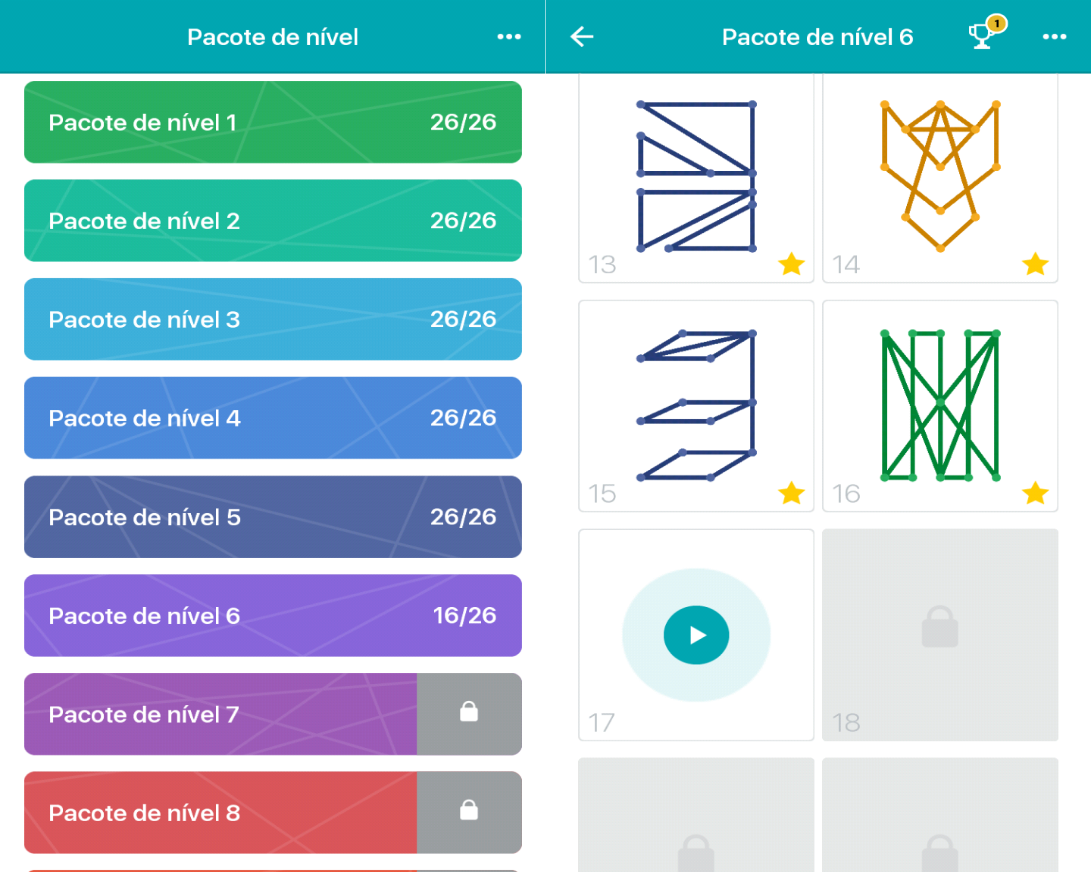
\includegraphics[width=0.5\linewidth]{img/niveisONELINE}
			\caption{Níveis no Jogo OneLine}
			Fonte: ONELINE
			\label{lvlOneLine}
		\end{figure}		
		A Figura \ref{lvlOneLine} mostra os níveis do jogo mobile OneLine.  Do lado esquerdo é mostrado os níveis principais e do lado direito pode-se observar os subníveis. O jogo tem como principal objetivo completar figuras com apenas uma linha e a cada nível a dificuldade aumenta.
		
		\subsubsection{Classificação}
		Segundo \citeonline{zichermann2011gamification}, a classificação tem por objetivo a comparação entre os jogadores. Uma tabela de classificação é facilmente entendida e geralmente é aprendida através de uma lista ordenada com o nome do jogador e a sua pontuação ao lado, podendo ter outros atributos relevantes do jogo.
		
		\citeonline{zichermann2011gamification} citam ainda que existem dois tipos de lista de classificação: A primeira é o quadro não desincentivo de lideres, que é mais uma classificação social, geralmente usada em redes sóciais e o outro tipo é o placar infinito, que é quando um jogador consegue chegar a um certo nível e fica no ranking em uma certa posição até que alguém o supere e tire seu lugar. Um jogador que demonstre interesse profundo em um posicionamento da tabela pode ser considerado competitivo.
		
		Às vezes, a comparação por meio de quadros de classificação pode ser uma tarefa bem complicada, por expor publicamente os jogadores e isso pode desestimular o jogador a continuar ativo no sistema gamificado. Por esse motivo, a criação de um ranking não é tão obvia como parece \cite{zichermann2011gamification}.
		
			\begin{figure}[H]
				\centering
				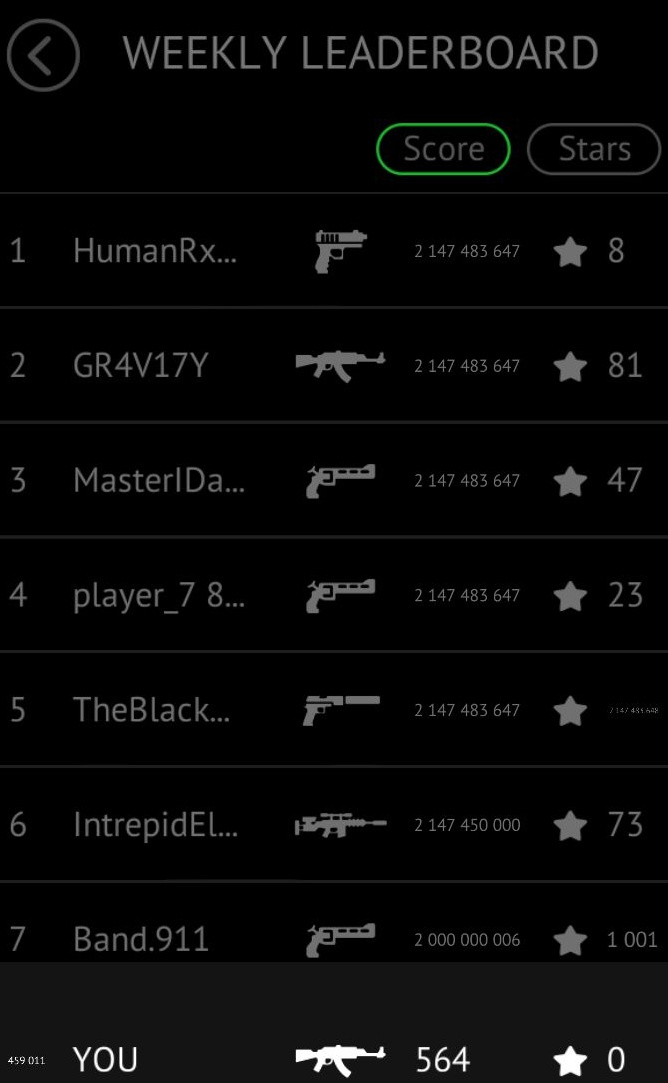
\includegraphics[width=0.3\linewidth]{img/ClassificacaoFLIPTHEGUN}
				\caption{Ranking Geral Jogo FlipTheGun}
				Fonte: FlipTheGun
				\label{flipthegunBadges}
		\end{figure}	
		A Figura \ref{flipthegunBadges} mostra a tabela de classificação global do jogo \textit{Flip The Gun}. Onde tem-se a classificação por pontuação dentro do jogo, a tabela mostra informações como: A classificação do jogador, o nome do mesmo, o tipo de arma que o jogador mais usa no jogo, sua pontuação total e por fim suas estrelas, que também é um tipo de pontuação dentro do jogo e é também é uma forma de classificação.
		
		\subsubsection{Emblemas}
		\citeonline{zichermann2011gamification} citam que os distintivos ou emblemas são muito presentes em nosso mundo, pois além de status, as pessoas os colecionam pelos mais diversos motivos e causas, e das mais diversas formas e esses distintivos servem para demonstrar para os outros jogadores  as conquistas realizadas pelo jogador que os possui ou para demonstrar e marcar a conclusão das metas estabelecidas.
		
		\citeonline{zichermann2011gamification}, ainda citam que em alguns sistemas gamificados os distintivos podem substituir os sistemas convencionais de níveis, porém há conceitos como \textit{badgenfreud} que sugere que uma grande quantidade de distintivos torna a experiência chata e sem sentido.
		
		\begin{figure}[H]
			\centering
			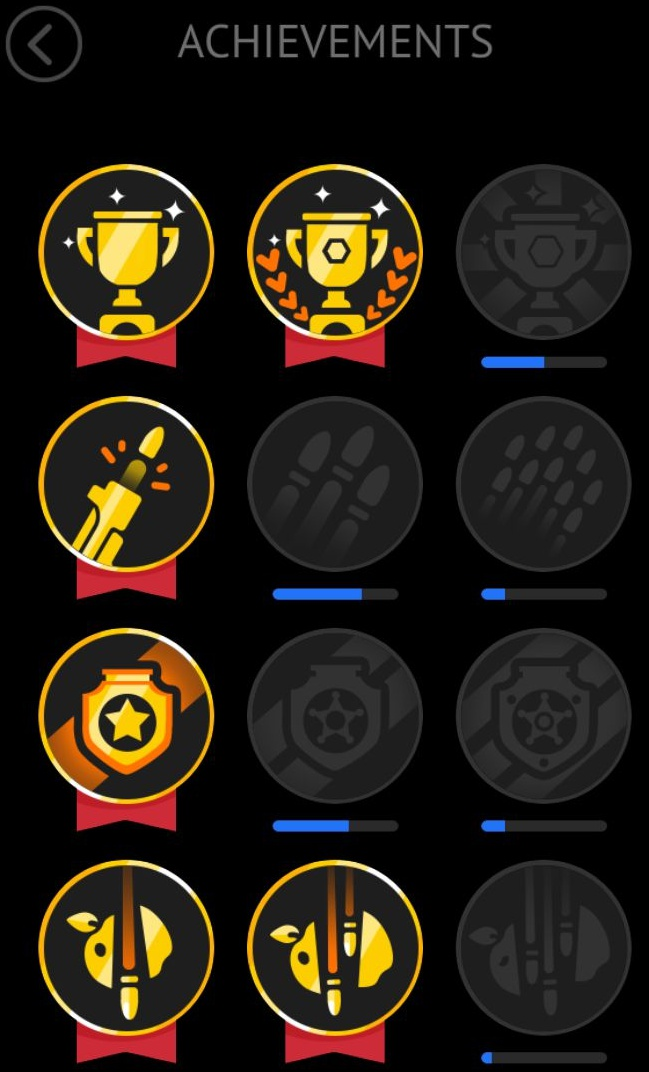
\includegraphics[width=0.3\linewidth]{img/EmblemasFLIPTHEGUN}
			\caption{Emblema do Jogo FlipTheGun}	
			Fonte: FlipTheGun
			\label{emblemasFlipTheGun}
	   \end{figure}	
   		A Figura \ref{emblemasFlipTheGun} traz os emblemas de conquista do jogo \textit{Flip The Gun}, para se conseguir qualquer um deles é preciso cumprir uma determinada meta ou missão que é dada pelo jogo.
		\subsubsection{Desafios}
		Para \citeonline{zichermann2011gamification}, em uma experiência gamificada, os desafios e as missões são uma forma de comunicar ao jogador o que ele deve fazer, algumas pessoas ao entrarem em um jogo, ou em uma experiencia gamificada, se veem perdidas e sem saber qual rumo tomar ou o que fazer, dessa forma os desafios e missões são uma forma de ajudá-los e guiá-los pela experiência.
		
		A ideia principal é que haja sempre um desafio para o jogador, alguns tipos de jogadores irão jogar os diversos desafios seguidos, tentando vencer o máximo deles da melhor forma possível, já outros tentarão somente a quantidade de desafios necessárias para aquele momento \cite{zichermann2011gamification}.
		
		Outro conceito importante é o de missões cooperativas, este conceito permite que uma comunidade de jogadores se reúna com a intenção de realizar uma determinada missão. Dessa forma, as missões cooperativas, além de promover um relacionamento entre os jogadores, deixam os jogos mais poderosos no quesito social \cite{zichermann2011gamification}.
		
		\begin{figure}[H]
			\centering
			\includegraphics[width=0.3\linewidth]{img/DesafiosSplashy}
			\caption{Desafios do Jogo Splashy}
			Fonte: Splashy
			\label{desafiosSplashy}
		\end{figure}	
				A Figura \ref{desafiosSplashy} mostra os desafios do jogo mobile Splashy, que tem por objetivo básico guiar uma bola sobre plataformas, esse jogo apresenta três tipos de desafios, e a cada novo desafio a dificuldade aumenta.
		\subsubsection{Integração}
		A integração se da pelo ato de levar e acolher um novato ao sistema gamificado, dessa forma o primeiro minuto de um jogo é considerado o mais importante, pelo fato de ser o momento em que o jogador toma as seguintes decisões: se gosta ou não do jogo, se vai ou não continuar no jogo, entre outras decisões importantes. O desenvolvedor, por esse motivo, deve maximizar os efeitos que o jogo causa sobre o jogador no primeiro minuto \cite{zichermann2011gamification}.
		
	\citeonline{zichermann2011gamification} citam que o primeiro minuto de jogo é o tempo em que o jogador experimenta o jogo. Um erro bastante comum, e que pode assustar o possível jogador, é pedir com que ele o se registre no inicio, sem ao menos dar tempo para se interessar pelo jogo.
		
		Não é bom que seja mostrada muitas informações e regras escritas, pois isso também pode assustar o possível jogador. Uma forma eficaz seria oferecendo uma introdução interativa às regras e que gere recompensas ao jogador \cite{zichermann2011gamification}.
	
		\begin{figure}[H]
			\centering
			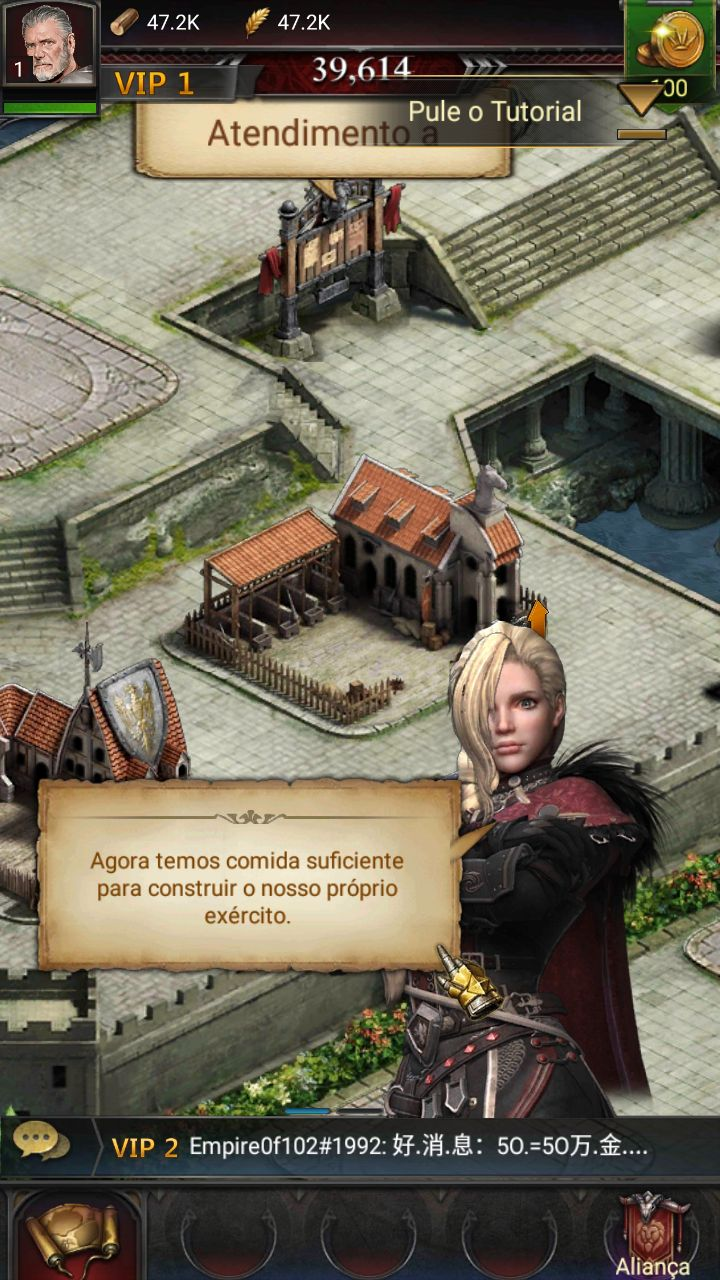
\includegraphics[width=0.3\linewidth]{img/tutorialCOK}
			\caption{Tutorial Clash Of Kings}
			Fonte: Clash Of Kings
			\label{tutorialCOK}
		\end{figure}
		Como foi descrito sobre a integração, a Figura \ref{tutorialCOK} demonstra o tutorial inicial do jogo \textit{mobile Clash Of Kings}, essa introdução serve para ensinar as mecânicas e dinâmicas do jogo, bem como, integrar e familiarizar com o ambiente em questão.
		
		\subsubsection{Engajamento}
		Para \citeonline{zichermann2011gamification}, o  desenvolvedor não deve apenas observar como o jogador está interagindo com o sistema gamificado, ele deve também observar como o jogo em questão ou experiência gamificada afeta o jogador emocionalmente, e o mais importante, o desenvolvedor deve observar e saber o que leva o jogador a voltar ao jogo.
		
		A melhor  forma de pensar na maneira de tornar um sistema gamificado viral e colocar as ações da Figura \ref{cicloEngajamento} em diversos pontos do sistema de jogo, é fazer com que o jogador sempre deseje voltar a jogar. É importante salientar que o engajamento no jogo sempre vai variar, dependendo do nível de conhecimento do jogador, por isso é importante buscar formas de motivar tanto jogadores mais experientes quanto os iniciantes \cite{zichermann2011gamification}.
		
		\begin{figure}[H]
			\centering
			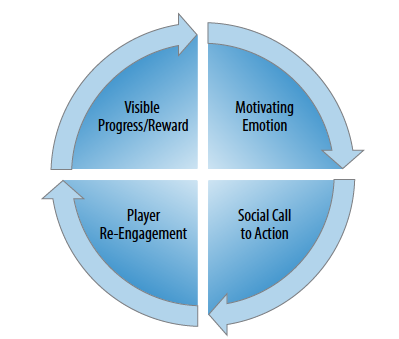
\includegraphics[width=0.5\linewidth]{img/loopdeengajamento}
			\caption{Ciclo de Engajamento}
			Fonte: Livro Gamification by design
			\label{cicloEngajamento}
		\end{figure}

		A Figura \ref{cicloEngajamento} demonstra os passos ou as partes do ciclo de engajamento segundo segundo \citeonline{zichermann2011gamification}.
		
\section{Considerações Finais}
Este capítulo discutiu os principais conceitos necessários a este trabalho. Foram apresentado conceitos a respeito do trastorno do espectro autista e formas de tratamento baseados em técnicas de aprendizado, bem como os conceitos e técnicas de e-learning e os principais conceitos e mecânicas da gamificação. A seguir será apresentado a metodologia usada para o desenvolvimento deste trabalho de estágio,  os trabalhos que apresentam a mesma temática deste trabalho e no que este se difere dos demais e os resultados obtidos durante a pesquisa.